\documentclass{scrartcl}
\usepackage{placeins}
\usepackage{longtable}
\usepackage{tabularx}
\usepackage{titlesec}

% zusätzliche mathematische Symbole, AMS=American Mathematical Society 
\usepackage{amssymb}
\usepackage{amsmath}

% fürs Einbinden von Graphiken
\usepackage{graphicx}

% für Namen etc. in Kopf- oder Fußzeile
\usepackage{fancyhdr}

% erlaubt benutzerdefinierte Kopfzeilen 
\pagestyle{fancy}

% Definition der Kopfzeile
\lhead{
\begin{tabular}{ll}
Emma Bach\\
\end{tabular}
}
\chead{}
\rhead{\today{}}
\lfoot{}
\cfoot{Seite \thepage}
\rfoot{} 

\titleformat{\section}[block]{\Huge\bfseries\filcenter}{}{}{}
\titleformat{\subsection}[block]{\Large\bfseries}{}{}{}
\titleformat{\subsubsection}[block]{\large\bfseries}{}{}{}

\newcommand{\Partial}[1]{\frac{\partial}{\partial #1}}

\begin{document}
\section*{Computer Graphics}
\subsection*{Ray Casting}
\begin{itemize}
    \item \textbf{Ray Casting} estimates the projection of a scene onto a sensor using ray intersections
    \item Challenge: Incoming and outgoing light at every point of the scene needs to be known (in theory)
    \item \begin{itemize}
        \item Primary rays solve the visibility Problem (What is visible?)
        \item The rendering equation / A Shading Model uses secondary rays solve color, brightness etc.
    \end{itemize}
    \item Ray Tracing: Function $L(p, \omega_i)$ gives Light at point $p$ coming from direction $\omega_i$
    \item Outgoing light in direction $\omega_o$ can then be calculated as a weighted sum/integral of the incoming rays
    \item Rays are specified as equation $r(t) = ot + d$
\end{itemize}
\subsection*{Implicit surfaces}
\begin{itemize}
    \item Defined as set of points $(x,y,z)$ such that $f(x,y,z) = 0$ for a given function $f$ 
    \item Ray intersects an implicit surface if $\exists t[f(r(t)) = 0]$
    \item For example: A plane in normal form is given by $n \cdot (p-r) = 0$, therefore the intersection with a ray is given by
    \begin{align*}
        n \cdot (o + td - r) = 0 \implies t = \frac{(r-o)\cdot n}{n \cdot d}
    \end{align*}
    Note that such an intersection only exists if $n$ ist not orthogonal to $d$, since otherwise $n \cdot d$ would be $0$.
    \item The surface normal of an implicit function $f$ at a point $p$ is given by the gradient
    \begin{align*}
        n_p = \nabla f(p) = \left(\Partial{x}f(p), \Partial{y}f(p), \Partial{z}f(p)\right)
    \end{align*}
\end{itemize}
\newpage
\subsubsection*{Quadrics}
\begin{itemize}
    \item Implicit surfaces given by quadratic equations, which means there can be at most two intersections with a given ray.
    \item Examples:
    \begin{itemize}
        \item Sphere: $\frac{x^2+y^2+z^2}{a^2}-1 = 0$
        \item Ellipsoid: $\frac{x^2}{a^2}+\frac{y^2}{b^2}+\frac{z^2}{c^2}-1 = 0$
        \item Paraboloid: $\frac{x^2+y^2}{a^2}-z=0$
        \item Hyperboloid: $\frac{x^2}{a^2}+\frac{y^2}{b^2}-\frac{z^2}{c^2}-1 = 0$
        \item Cone: $\frac{x^2}{a^2}+\frac{y^2}{b^2}-\frac{z^2}{c^2} = 0$
        \item Cylinder: $\frac{x^2+y^2}{a^2}-1=0$
    \end{itemize}
\end{itemize}
\subsection*{Parametric surfaces}
\begin{itemize}
    \item Given by set of equations with two parameters:
    \begin{align*}
        x = f(u,v), y = g(u,v), z = h(u,v)
    \end{align*}
    \item Normal vector is given by:
    \begin{align*}
        n_{u,v} = \left(\Partial{u}f(u,v), \Partial{u}g(u,v), \Partial{u}h(u,v)\right) \times \left(\Partial{v}f(u,v), \Partial{v}g(u,v), \Partial{v}h(u,v)\right)
    \end{align*}
    \item Examples:
    \begin{itemize}
        \item Cylinder, with parameters $\phi \in [0, 2\pi)$ and $v \in [0,1]$: 
        \begin{align*}
            x = \cos(\phi),\ y = \sin(\phi),\ z = z_{min} + v(z_{max} - z_{min})
        \end{align*}
        \item Sphere, with parameters $\phi \in [0, 2\pi)$ and $\theta \in (0,\pi]$
        \begin{align*}
            x = \cos(\phi)\sin(\theta),\ y = \sin(\phi)\sin(\theta),\ z = \cos(\theta)
        \end{align*}
        \item Discs
        \item Cones
    \end{itemize}
    \item Can be used to render partial objects by restricting the range of the parameters
\end{itemize}
\subsection*{Combined Objects}
\begin{itemize}
    \item Constructive Solid Geometry (CSG): Combine objects using boolean operators
    \item Only for closed surfaces with defined volumes
    \item \textbf{Union} $A \cup B$: Closest intersection with either, \textbf{Intersection} $A \cap B$: Closest intersection with $A$ that is inside $B$ or vice versa, \textbf{Difference} $A \ B$: Closest intersection with $A$ that is not in $B$
\end{itemize}
\subsection*{Triangles}
\begin{itemize}
    \item Given parametrically by:
    \begin{align*}
        p(b_1, b_2) = (1-b_1-b_2)p_0 + b_1 p_1 + b_2 p_2
    \end{align*}
    Where $p_0, p_1, p_2$ are the vertices of the triangle and $b_1 \geq 0$, $b_2 \geq 0$, $b_1 + b_2 \leq 1$
\end{itemize}
\subsection*{Box Tests}
\begin{itemize}
    \item Intersection test with simple geometry around complex geometry, so that rays that completely miss the mark can be discarded quickly and efficiently
    \item Generally combined into trees of progressively smaller / more accurate boxes - if ray intersects a box, check intersections with small boxes inside that box
\end{itemize}
\subsection*{Iso-Surfaces in Grids}
\begin{itemize}
    \item Fluid Particles -> Density Values on a grid -> 
\end{itemize}
\subsection*{Rendering}
\begin{itemize}
    \item \textbf{Colored Light} represented as $3$-dimensional Vector with red, green, and blue components
    \item Surface color is characterized by how much of each color the surface absorbs / reflects
    \item \textbf{Rendering Equation}:
    \begin{align*}
        L(p, \omega_o) = \int_{i} \text{mat}(p, \omega_i, \omega_o)L(p, \omega_i)\cos(\theta_i)d\omega_i
    \end{align*}
    So: Outgoing Light is equal to the sum / integral of incoming light from all directions, weighted by the material properties of the material involving light from that direction going into the other direction, times the cosine of the angle between incoming and outgoing light
\end{itemize}
\subsubsection*{Shading Models}
\begin{itemize}
    \item Light coming from a point is calculated only considering direct illumination.
    \begin{align*}
        L(p,\omega_o) = \sum_{i \in I} f(L(p,\omega_i))   
    \end{align*}
    Where $I$ ist the set of light sources and $f$ is a function given by the particular rendering model.
    \item \textbf{Lamberts cosine Law}:
    \begin{align*}
        L(p,\omega_o) = L(p, \omega_i)\cos(\theta_i)
    \end{align*}
    \item \textbf{Phong illumination model:}
    \begin{align*}
        L(p,\omega_o) &= L_\text{Ambient} + L_\text{Diffuse} + L_\text{Specular}\\
        &= \alpha \cdot \rho \otimes L_\text{Indirect} + \sum_{i \in I} L_i \cdot (n \cdot l_i) \otimes (\beta \cdot \rho + \gamma \cdot \rho_{\text{White}} \cdot (r_i \cdot v)^m)
    \end{align*}
    Where:
    \begin{itemize}
        \item $\otimes$ is componentwise multiplication
        \item $\rho$ is the color of the surface at the given point
        \item $L_i$ is the light given off by light source $i$
        \item $l_i$ is the normalized vector pointing from the given point to light source $i$
        \item $n$ is the surface normal at the given point
        \item $\theta_i$ is the angle between $l_i$ and $n$
        \item $r_i = 2 \cdot \cos(\theta_i) \cdot n - l_i$, the vector $l_i$ "reflected" along $n$
        \item $v$ is the normalized vector pointing from the given point to the sensor
        \item $\alpha, \beta$ and $\gamma$ are user-defined scalar coefficients describing the strength of Ambient, Diffuse, and Specular Lighting.
        \item $m$ describes the size and brightness of the specular highlight
    \end{itemize}
    \item The Phong model is limited to opaque surfaces. Reflective or transparent surfaces are not considered.
    \item The Phong model is not physical, i.e. conservation of energy is generally not respected
\end{itemize}
\subsubsection*{Extensions of the Phong Model}
\begin{itemize}
    \item \textbf{Considering Distances:} The light at a given surfaces is inversely proportional to the distance to the light source. 
    \begin{align*}
        L^\text{Surf}_i = \frac{1}{d^2} L_i \cdot (n \cdot l)    
    \end{align*}
    \item \textbf{Fog}: Linear interpolation between computed Light $L_\text{cam}$ and fog color $c_f$. 
    \begin{align*}
        L = f(d) L_\text{cam} + (1-f(d))c_f    
    \end{align*}, where $d$ is the distance from the point to the viewer and $f$ is some function describing light weakening as it travels through fog, for example $f(d) = \frac{a-d}{a-b}$ for constants $a,b$
\end{itemize}
\subsubsection*{Other shading models}
\begin{itemize}
    \item Shading models can be evaluated per fragment (i.e. Pixel) or per vertex
    \item \textbf{Flat shading}: Fragments are colored with the color of one specific vertex, very efficient
    \item \textbf{Gouraud shading}: Fragment colors are interpolated from vertext colors. Cheaper than Phong, mach band effect, local highlights may still be lost
    \item \textbf{Phong shading}: Evaluation per Fragment, using normals interpolated from the vertex normals, more costly
\end{itemize}
\subsection*{Homogeneous Notation}
\begin{itemize}
    \item Allows translation to be expressed as a linear transformation and therefore as a simple matrix multiplication
    \item The \textbf{Model transform} $M_m$ transforms from a model $m$'s Local coordinate system to the global coordinate system
    \item The \textbf{View transform} $V$ transforms from the camera's local coordinate system (with the camera at the origin facing one of the coordinate axes) to the global coordinate system
    \item The \textbf{Inverse View Transform} $V^{-1}$ is applied to all objects in order to translate the entire system into \textbf{View Space / Camera Space}, with the camera aligned at the origin as previously mentioned.
    \item In order to directly translate from local space to view space, the modelview transform $V^{-1}M_m$ is applied. In the case of the camera, this means the modelview transform is simply the identity matrix.
    \item In \textbf{homogeneous Notation}, the position $(\frac{x}{w},\frac{y}{w},\frac{z}{w})$ is represented as $(x,y,z,w)$, with scalar multiples of this vector representing the same position.
    \item Positions of the form $(x,y,z,0)$ represent positions at infinity. In practice this is usually used to represent directional vectors as positions.
    \item Arbitrary affine transformations can now be realized through matrices of the form
    \begin{align*}
        \begin{pmatrix}
            m_{00} & m_{01} & m_{02} & t_0\\
            m_{10} & m_{11} & m_{12} & t_1\\
            m_{20} & m_{21} & m_{22} & t_2\\
            p_{0} & p_{1} & p_{2} & w\\
        \end{pmatrix}
    \end{align*}
    Where $m$ represents ordinary linear transformations (shear, scale, rotation), $t$ represents translation and $p$ represents projection. If $p_2$ is $0$, we have parallel projection (Viewpoint is at infinity), otherwise we have perspective projection. Parallel projection can be orthographic or oblique, perspective projection can involve one vanishing point or two.
    \item The inverse of a rotation matrix is its transpose.
    \item Rotation and reflection matrices are orthogonal
    \item Rotation matrices have determinant $1$ and reflection matrices have determinant $-1$
    \item Combinations of rotation and translation (i.e. rotations, including rotation around infinity) are known as \textbf{Rigid-Body Transforms}
    \item Scalar multiples of a projection represent the same projection.
    \item Parallel projections can simply be realized as identity matrices with one of the $1$s changed into a $0$.
    \item The \textbf{Projection transform} $P$ transform view space (a frustum, with "correct" corner coordinates) into \textbf{Clip Space / NDC Space} (a cube, with corners (1,1), (-1,-1) etc, known as the \textbf{Canonical view volume}). It is given by
    \begin{align*}
        P = 
        \begin{pmatrix}
            \frac{2n}{r-l} & 0 & -\frac{r+l}{r-l} & 0\\
            0 & \frac{2n}{t-b} & -\frac{t+b}{t-b} & 0\\
            0 & 0 & \frac{f+n}{f-n} & -\frac{2fn}{f-n}\\
            0 & 0 & 1 & 0\\
        \end{pmatrix}
    \end{align*}
    Where the constants refer to the coordinates of the corners (left, right, top, bottom, near, far)
    \item For $t = -b$ and $l = -r$ this simplifies to
    \begin{align*}
        P = 
        \begin{pmatrix}
            \frac{n}{r} & 0 & 0 & 0\\
            0 & \frac{n}{t} & 0 & 0\\
            0 & 0 & \frac{f+n}{f-n} & -\frac{2fn}{f-n}\\
            0 & 0 & 1 & 0\\
        \end{pmatrix}
    \end{align*}
    \item Can end up looking strange if near plane is too close to zero
\end{itemize}
\subsection*{Rasterization}
\begin{itemize}
    \item Local Space $-\ PV^{-1} M_i \to$ Canonical view volume $\to$ Rasterization $\to$ Visibility Tests $\to$ Shading $\to$ finished image
    \item Fragment = Candidate for a pixel, Primitive = Line
\end{itemize}
\subsubsection*{Vertex Processing}
\begin{itemize}
    \item Input: Vertices
    \item Output: Vertices
    \item Computation of Vertex Positions, Color, Texture positions etc.
    \item Transformation from local space to the canonical view volume ($PV^{-1}M_i$)
\end{itemize}
\subsubsection*{Rasterization}
\begin{itemize}
    \item Input: Vertices
    \item Output: Fragments
    \item Sets or interpolates fragment attributes using vertex attributes
    \item Polygon Rasterization: Compute intersections with horizontal scanlines $y = y_i + 0.5$, fill positions between intersections with fragments
    \item Fragment attributes are interpolated from Vertex attributes
\end{itemize}
\subsubsection*{Fragment Processing}
\begin{itemize}
    \item Input: Fragments
    \item Output: Fragments
    \item Processes fragment attributes, discards fragments that are not visible
    \item Texturing, Fog, Antialiasing, $\hdots$
    \item \textbf{Scissor Test:} Test if fragment is inside specified rectangle
    \item \textbf{Alpha Test:} Transparency, Billboarding (Sprite that always faces the camera)
    \item \textbf{Stencil Test:} Used for shadows etc.
    \item \textbf{Depth Test:} Are any new fragments behind fragments that are already rendered?
\end{itemize}
\subsubsection*{Framebuffer Update}
\begin{itemize}
    \item Get updated framebuffer attributes from processed fragments
    \item Overwrite old fragment if not transparent, otherwise if alpha < 1 combine old fragment color with new fragment color weighted by the alpha value
\end{itemize}
\subsection*{Curves}
\begin{itemize}
    \item Defined by parametric functions $x(t), y(t), z(t)$
    \item For \textbf{rational curves}, these functions have the form $\frac{p(t)}{q(t)}$ with $p$ and $q$ being polynomials
    \item Bezier Curves: Functions are linear interpolations of linear interpolations
    \item As a result, a degree $n$ bezier curve has the form 
    \begin{align*}
        \sum (1-t)^it^jp_k   
    \end{align*} for $i+j = n$, with $p_k$ being the control points.
    For example, for a quadratic bezier curve, the function is:
    \begin{align*}
        q(t) &= (1-t)[(1-t)p_0 + tp_1] + t[(1-t)p_1 + tp_2]\\
        &= (1-t)^2p_0 + 2(1-t)tp_1 + t^2p_2
    \end{align*}
    and for a cubic bezier curve, the function is:
    \begin{align*}
        c(t) = (1-t)&[(1-t)[(1-t)p_0 + tp_1] + t[(1-t)p_1 + tp_2]]\\
        +  t&[(1-t)[(1-t)p_1 + tp_2] + t[(1-t)p_2 + tp_3]]\\
        = (1-t)^3&p_0 + 3(1-t)^2tp_1 + 3(1-t)t^2p_2 + t^3p_3
    \end{align*}
    \item The exact general formula for a degree $n$ bezier curve is:
    \begin{align*}
        \sum^{n}_{i=0} B_{i,n}(t)p_i
    \end{align*}
    Where $B_{i,n}$ are the so-called \textbf{Bernstein Polynomials}
    \begin{align*}
        B_{i,n}(t) = \binom{n}{i}(1-t)^{n-i}t^i
    \end{align*}
    In Praxis, curves of degree greater than $3$ are only rarely used, because the control points are a lot more difficult to get right.
    \item \textbf{Properties of Bernstein Polynomials}:
    \begin{itemize}
        \item Partition of Unity: 
        \begin{align*}
            \sum^{n}_{i=0} B_{i,n}(t) = 1
        \end{align*}
        \item Positivity:
        \begin{align*}
            B_{i,n}(t) \geq 0
        \end{align*}
        \item Symmetry:
        \begin{align*}
            B_{i,n}(t) = B_{n-i,n}(1-t)
        \end{align*}
        \item Recursive definition:
        \begin{align*}
            B_{i,n}(t) = (1-t)B_{i,n-1}(t) + tB_{i-1,n-1}(t)
        \end{align*}
        \item Endpoint Interpolation:
        \begin{align*}
            x(0) = p_0, x(1) = p_n
        \end{align*}
        \item Endpoint Tangent:
        \begin{align*}
            \frac{d}{dt} x(0) = n(p_1-p_0), \frac{d}{dt} x(1) = n(p_n-p_{n-1})
        \end{align*}
    \end{itemize}
    \item $x(t)$ is part of the smallest convex set that contains all control points (the \textbf{convex hull}), i.e. if you draw lines between every control point, the bezier curve is contained fully inside the resulting shape.
    \item An affine transformation can be applied to a bezier curve by applying it to the control points.
    \item Every control point affects the entire bezier curve, just weighted at each point by the Bernstein Polynomials.
    \item General formulation of a \textbf{Spline} of degree $n$:
    \begin{align*}
        x(t) = GST(t)
    \end{align*}
    Curve = Geometry Matrix (Control Points) $\cdot$ Spline Matrix $\cdot$ Basis (Standard Polynomial Basis)
    For a 2D degree 3 bezier curve with control points $\binom{p_i}{q_i}$, this ends up being:
    \begin{align*}
        \begin{pmatrix}
            x(t) \\ y(t)
        \end{pmatrix}
        =
        \begin{pmatrix}
            p_0 & p_1 & p_2 & p_3 \\ q_0 & q_1 & q_2 & q_3
        \end{pmatrix}
        \begin{pmatrix}
            1 & -3 & 3 & -1\\
            0 & 3 & -6 & 3\\
            0 & 0 & 3 & -3\\
            0 & 0 & 0 & 1\\
        \end{pmatrix}
        \begin{pmatrix}
            1 \\ t \\ t^2 \\ t^3
        \end{pmatrix}
    \end{align*}
    \item a 3D cubic bezier curve can be realized by simply replacing the geometry matrix with
    \begin{align*}
        \begin{pmatrix}
            p_0 & p_1 & p_2 & p_3 \\ q_0 & q_1 & q_2 & q_3\\ r_0 & r_1 & r_2 & r_3
        \end{pmatrix}   
    \end{align*}
    \item Bezier Curves can be subdivided using the \textbf{De Casteljau} algorithm
    \item A parametric curve is $C^k$-continuus if the first $k$ derivatives of $x(t), y(t)$ etc. exist and are continuous
    \item A cubic bezier curve with end points $p_i$ and $p_{i+1}$ and end velocities $m_i$ and $m_{i+1}$ is given by
    \begin{align*}
        x^i(t) = p_iH_{0,3}(t)+p_iH_{1,3}(t) + m_iH_{2,3}(t) + m_{i+1}H_{3,3}(t)
    \end{align*}
    Where $H_{i,n}$ are the cubic hermite basis functions:
    \begin{align*}
        H_{0,3}(t) &= 1 - 3t^2 + 2t^3 = B_{0,3}(t) + B_{1,3}(t)\\
        H_{1,3}(t) &= 3t^2 - 2t^3 = B_{2,3}(t) + B_{3,3}(t)\\
        H_{2,3}(t) &= t - 2t^2 + t^3 = \frac{1}{3}B_{1,3}(t)\\
        H_{3,3}(t) &= -t^2 + t^3 = -\frac{1}{3}B_{2,3}(t)\\
    \end{align*}
    \item \textbf{Catmull-Rom Splines} are a variant of Hermite Splines where $m_i = \frac{1}{2}(p_{i+1} - p_{i-1})$ and $m_{i+1} = \frac{1}{2}(p_{i+2} - p_{i})$ (So derivatives are given by new, additional control points $p_{i-1}$ and $p_{i+2}$)
\end{itemize}
\subsection*{Particle Fluids}
\begin{itemize}
    \item \textbf{Explicit Euler:} 
    \begin{align*}
        x^{t+h} = x^t + hv^t + O(h^2)\\
        v^{t+h} = v^t + ha^t + O(h^2)\\
    \end{align*}
    \item Alternative Taylor approximation:
    \begin{align*}
        x^{t+h} = x^t + hv^t  + \frac{h^2}{2}a^t + \frac{h^3}{6}\frac{d}{dt}a^t + O(h^4)
    \end{align*}
    \item \textbf{Navier-Stokes-Equation:}
    \begin{align*}
        a_i^t = -\frac{1}{\rho_i^t}\nabla p_i^t + \nu\nabla^2 v_i^t + \frac{F_i^t}{m_i}
    \end{align*}
    Where:
    \begin{itemize}
        \item $\rho$ is the density, $p$ is the pressure and $\nu$ is the viscosity
        \item $-\frac{1}{\rho_i^t}$ represents acceleration due to pressure differences
        \item $\nu\nabla^2 v_i^t$ represents Acceleration due to friction between particles of different velocities
        \item $\frac{F_i^t}{m_i}$ represents outside forces such as gravity
    \end{itemize}
\end{itemize}
\subsubsection*{Smoothed Particle Hydrodynamics (SPH)}
\begin{itemize}
    \item Interpolates quantities at arbitrary positions and approximates derivatives with adjacent particles
    \item Can be used to compute $\rho_i^t$, $-\frac{1}{\rho_i^t}\nabla p_i^t$, $\nu\nabla^2 v_i^t$ and $\frac{F_i^t}{m_i}$
    \item Quantity $A_i$ at an arbitrary position $x_i$ is calculated by sampling known values $A_j$ at positions $x_j$:
    \begin{align*}
        A_i = \sum_j A_j \frac{m_j}{\rho_j}W_{ij}
    \end{align*}
    where $W_{ij}$ is a function that weighs contributions of positions based on their distance to $x_i$, for example a gaussian distribution.
    \item 
    \begin{align*}
        \nabla A_i = \sum_j A_j \frac{m_j}{\rho_j}\nabla W_{ij}
    \end{align*}
    \item For example, the density can now be calculated through the \textbf{Explicit SPH Form} as:
    \begin{align*}
        \rho_i &= \sum_j \rho_i \frac{m_j}{\rho_j}W_{ij}\\
        &= \sum_j m_jW_{ij}
    \end{align*}
    \item Pressure calculation:
    \begin{align*}
        p_i = \max\left(k\left(\frac{\rho_i}{\rho_0} -1\right), 0\right)
    \end{align*}
    For resting pressure $\rho_0$ and a user-defined stiffness $k$
    \item Pressure acceleration in SPH:
    \begin{align*}
       a_i^p &= -\frac{1}{\rho_i}\nabla p_i\\
       &= -\sum_j m_j \left(\frac{p_i}{\rho_i^2}+\frac{p_j}{\rho_j^2}\right)\nabla W_{ij}
    \end{align*}
    \item Viscosity acceleration in SPH:
    \begin{align*}
        \nu\nabla^2 v_i^t = 2\nu\sum_j \frac{m_j}{\rho_j} \frac{v_{ij} \cdot x_{ij}}{x_{ij} \cdot x_{ij} + 0.01h^2} \nabla W_{ij}
    \end{align*}
\end{itemize}
\subsubsection*{Neighbor Search}
\begin{itemize}
    \item Particles are stored in a grid
    \item Edge length equal to the radius of the kernel function
    \item Compute unique identifier for each particles (for example via space filling curves)
    \item Sort particles by identifier and store in a hash table
\end{itemize}
\subsubsection*{Boundaries}
\begin{itemize}
    \item Boundaries are represented as particles that still contribute to density, pressure and pressure acceleration
    \item Boundary particles are static fluid particles
\end{itemize}
\subsubsection*{Iso-Surface-Reconstruction (Marching Cubes)}
\begin{itemize}
    \item Initialize density values at points on grid using SPH
    \item $\rho_i < \rho_0$ $\to$ Particle outside the fluid, $\rho_i \approxeq \rho_0$ $\to$ Particle inside the fluid
    \item Generate Outline around grid points that are in the fluid using triangle lookup tables
\end{itemize}
\newpage
\section*{Image Processing}
(Chapter 1 and 2 skipped)
\subsection*{Energy Minimization}
\begin{itemize}
    \item Formulate a Task as a minimization problem
    \item The function $E(x)$ whose minimum you want to find is often called the \textbf{Energy Function}, or in machine learning the \textbf{Loss Function}
    \item First step is to formulate assumptions:
    \begin{itemize}
        \item Similarity to the input image, so minimize
            \begin{align*}
                E_D(u_{i,j}) := \sum_{i,j} (u_{i,j} - I_{i,j})^2
            \end{align*}
        \item Similarity to neighboring values (smoothness), so minimize
            \begin{align*}
                E_S(u_{i,j}) := \sum_{i,j} (u_{i+1,j} - u_{i,j})^2 + (u_{i,j+1} - u_{i,j})^2
            \end{align*}
    \end{itemize}
    \item Now solve the problem of minimizing $aE_D(u_{i,j}) + bE_S(u_{i,j})$, where $a$ and $b$ are weighting parameters
    \item Advantages:
    \begin{itemize}
        \item Transparency (Clearly stated assumptions)
        \item Optimality (Provably optimal under stated assumptions)
        \item Easy to analyze aspects of the problem
        \item Fewer Parameters than heuristic methods
        \item Compatible with other approaches
    \end{itemize}
    \item Advantages:
    \begin{itemize}
        \item Metrics can still be somewhat arbitrary - why minimize the squares? (Probabilistic arguments can help here)
        \item Choosing weight parameters is not easy (But can be optimized via a validation dataset)
        \item Often difficult in practice.
    \end{itemize}
    \item Actually solving the example problem means solving a very large system of linear equations involving a sparse matrix
    \item Positive definite Matrices, which we have here, always have an inverse.
    \item \textbf{Convex functions} have a positive second derivative. They always have a unique global minimum and no local minima. Can be minimized by solving $f'(x) = 0$ or through gradient descent.
    \item Any linear interpolation (= "convex combination") of convex functions is again convex.
    \item Actually solving the Matrix:
    \begin{itemize}
        \item \textbf{Jacobi Method} - Simple, parallelizable, but converges slowly and cant be computed in-place.
        \item \textbf{Gauss-Seidel, SOR} - Faster convergence, in place
        \item \textbf{Conjugate Gradient} - Convergence in a finite number of steps
        \item \textbf{Multigrid Methods} - Sometimes much faster
    \end{itemize}
    \item \textbf{Jacobi Method}:
    \begin{itemize}
        \item Decompose $A$ into its diagonal Part $D$ and off-diagonal Part $M$ ($A = D+M)$
        \item $Ax = b \Leftrightarrow (D+M)x = b \Leftrightarrow Dx = b - Mx$
        \item $D$ can be trivially inverted by inverting every entry
        \item Now start with any guess $x_0$ and iteratively calculate a new value $x_{i+1}$ as:
        \begin{align*}
            x_{i+1} = D^{-1}(b - Mx_i)    
        \end{align*}
        \item Iterate until either $Ax - b$ (also known as the residual, $r^k$) or $(x_{i+1}-x_i)^2$ is small enough 
    \end{itemize}
    \item \textbf{Gauss-Seidel Method}:
    \begin{itemize}
        \item Split $M$ into upper triangle $U$ and lower triangle $L$
        \item Now $Dx = b - Lx - Ux$
        \item During iteration, traverse $x$ from top to bottom. This way the new values can immediately be used in the multiplication with $L$:
        \begin{align*}
            x_{i+1} = D^{-1}(b - Lx_{i+1} - Ux_i)
        \end{align*}
        \item This leads to faster propagation of information and thus faster convergence
        \item Converges only if $A$ is positive or negative definite
    \end{itemize}
    \item \textbf{Successive Overrelaxation (SOR):}
    \begin{itemize}
        \item Add parameter $\omega$ to Gauss-Seidel which intentionally overshoots the answer:
        \begin{align*}
            x_{i+1} = (1-\omega)x^k + \omega D^{-1}(b - Lx_{i+1} - Ux_i)
        \end{align*}
        \item Optimal $\omega$ must be determined empirically.
    \end{itemize}
    \item \textbf{Conjugate Gradient (CG):}
    \begin{itemize}
        \item $u$ and $v$ are conjugate with respect to $A$ if 
        \begin{align*}
            \langle u,v \rangle_A := u^t A v = 0 
        \end{align*}
        \item Any set of $n$ conjugate vectors $\{p_k\}$ forms a basis of $\mathbb{R}^n$, so the solution $x$ of $Ax = b$ can be written as $x = a_1p_1 + \hdots + a_np_n$
        \item Then:
        \begin{align*}
            Ax &= \sum_{i=0}^n a_i A p_i\\
            \implies p_k^\top Ax &= \sum_{i=0}^n p_k^\top a_i A p_i = p_k^\top b\\
            \implies a_k &= \frac{p_k^\top b}{p_k^\top A p_k}
        \end{align*}
        \item This way an exact solution can be obtained in only $n$ computations.
        \item Obtaining the Basis:
        \begin{itemize}
            \item Start with arbitrary $x_0$
            \item $p_0 = r_0 = b - Ax_0$
            \item This is the gradient of 
            \begin{align*}
                E(x) = \frac{1}{2}x^\top Ax - b^\top x
            \end{align*}
            which is minimized by the solution $x$.
            \item Now iteratively compute:
            \begin{align*}
                a_k &= \frac{r_k^\top r_k}{p_k^\top A p_k}\\
                x_{k+1} &= x_k  + a_k p_k\\
                r_{k+1} &= r_k - a_k A p_k\\
                b_k &=  \frac{r_{k+1}^\top r_{k+1}}{r_k^\top r_k}\\
                p_{k+1} &= r_{k+1} + b_k p_k\\
            \end{align*}
            \item Stop when $r_k$ is small, guaranteed solution after $n$ iterations.
        \end{itemize}
        \item $A$ must be symmetric and positive definite
        \item In image processing, $n$ is the number of pixels, so an exact solution is usually not feasible
    \end{itemize}
    \item For all of these methods, the speed of convergence depends on the difference between the smallest and largest eigenvalues of $A$ (The \textbf{condition number})
    \item The condition number can be reduced through pre-conditioners $P^{-1}$ - instead of $Ax = b$, calculate $P^{-1}Ax = P^{-1}b$. The simplest preconditioner is the Jacobi Preconditioner, where $P = D$
    \item All of these methods have the disadvantage of only acting locally, because of the sparcity of the matrix. This problem can be solved by using a \textbf{Multigrid Solver}:
    \begin{itemize}
        \item A \textbf{unidirectional Multigrid} creates downsampled versions of the linear system by downsampling the image and deriving a new system from that.
        \item Use one of the previous methods to compute a first approximate solution from the downsampled image
        \item Upsample the solution and use this as the initial guess for solving the finer grid
        \item Advantages: Solving the coarse image is very fast, simple to implement
        \item Disadvantage: The coarse system doesn't always approximate the original system very well
        \item \textbf{Bidirectional Multigrid}: Downsample the error, not the image
        \begin{figure}[h!]
            \centering
            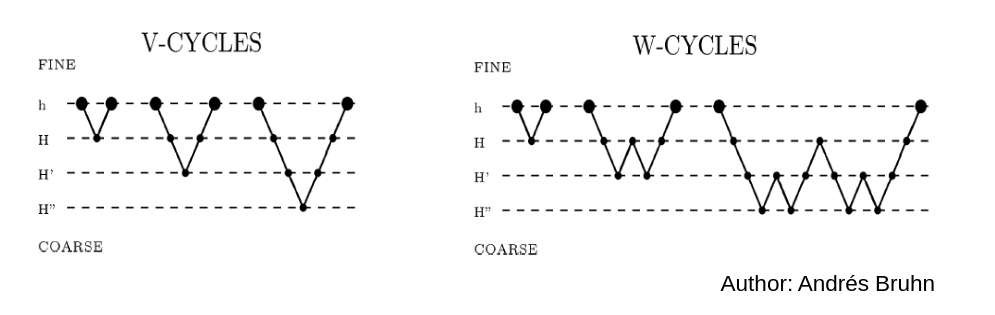
\includegraphics[width=0.9\linewidth]{bidirectionalmultigrid.png}
        \end{figure}
        \item Compute first solution at a fine grid:
        \begin{itemize}
            \item Run some iterations solving $A_hx_h = b_h$ on the fine grid
            \item This yields an approximate solution $x'_h$
            \item The remaining error is $e_h x_h - x'_h$
        \end{itemize}
        \item Correct error at a coarser grid:
        \begin{itemize}
            \item Approximate $e_h$, which is a solution of $A_h e_h = r_h$ ($r = b - Ax')$, by solving the system on the coarser grid ($A_H e_H = r_H$)
            \item Obtain better solution $x_h'' = x_h' + e_h$
        \end{itemize}
        \item Refine solution at a finer grid
        \begin{itemize}
            \item Run further iterations on the fine grid to decrease remaining error
        \end{itemize}
        \item \textbf{Full Multigrid}:
        \begin{itemize}
            \item Start at coarse grid, apply a full W-cycle at each finer level
        \end{itemize}
    \end{itemize}
\end{itemize}
\subsection*{Motion Estimation}
\begin{itemize}
    \item Goal: Find a vector field $(u,v)(x,y,t)$ that describes the motion of every point at every frame of a video. This video is called \textbf{optical flow}.
    \item Importance of optical flow:
    \begin{itemize}
        \item Can help with detection, segmentation and labeling of objects (\textbf{motion segmentation})
        \item Can be used to estimate 3D motion of objects (\textbf{scene flow})
        \item Can help estimate the 3D structure of objects (\textbf{structure from motion})
    \end{itemize}
    \item Assumption: Neighboring Pixels move the same way
    \item Otherwise, motion isnt clear - any pixel could have moved to any similarly colored pixel (This is known as the \textbf{aperture problem})
    \item Another common assumption: Gray value of a moving pixel stays constant:
    \begin{align*}
        I(x+u,y+v,t+1) - I(x,y,t) = 0
    \end{align*}
    \item This constraint is nonlinear, which makes estimation difficult.
    \item To make the problem easier, the first expression can be linearized through a taylor expansion:
    \begin{align*}
        I(x+u,y+v.t+1) = I(x,y,t) + I_x u + I_y v + I_t + O(u^2,v^2)
    \end{align*}
    Where $I_x = \frac{d}{dx}I(x,y,t)$
    \item This leads to the so-called \textbf{linearized optic flow constraint:}
    \begin{align*}
        I_x u + I_y v + I_t = 0
    \end{align*}
    This is precise if the images are smooth and the flow is small.
    \item The aperture problem is already visible here - there is one equation, but two unknowns. Therefore, it is impossible to find a unique flow vector.
    \item A second assumption is needed.
    \subsubsection*{The Lucas-Kanade Method}
    \item The \textbf{Lucas-Kanade method} assumes constant motion within a local neighborhood. This leads to the following system of equations:
    \begin{align*}
        I_x(x',y',t)u + I_y(x'+y',t)v+ I_t(x',y',t) = 0 \forall x' \forall y' \in \mathcal{R}(x,y)
    \end{align*}
    (for all $x',y'$ in a neighborhood around $(x,y)$)
    \item In general, this system is over-determined and doesn't have a solution. Instead, we try to minimize the squared error:
    \begin{align*}
        \text{argmin}_{u,v} \sum_{(x,y) \in \mathcal{R}} (I_x(x,y)u + I_y(x,y)v + I_t(x,y))^2
    \end{align*}
    \item Necessary conditions for a minimum are:
    \begin{align*}
        \Partial{u}E = 2\sum_{(x,y) \in \mathcal{R}} (I_x(x,y)u + I_y(x,y)v + I_t(x,y))I_x(x,y) = 0\\
        \Partial{v}E = 2\sum_{(x,y) \in \mathcal{R}} (I_x(x,y)u + I_y(x,y)v + I_t(x,y))I_y(x,y) = 0
    \end{align*}
    \item This leads to the following linear system at each pixel:
    \begin{align*}
        \begin{pmatrix}
            \sum I_x^2 & \sum I_x I_y\\
            \sum I_x I_y & \sum I_y ^2
        \end{pmatrix}
        \begin{pmatrix}
            u \\ v
        \end{pmatrix}
        = 
        \begin{pmatrix}
            -\sum I_x I_t\\
            -\sum I_y I_t\\
        \end{pmatrix}
    \end{align*}
    \item Can also use an arbitrary kernel function (usually a gaussian) instead of the previous uniformly weighted box. In this case, the sums come down to a convolution:
    \begin{align*}
        \begin{pmatrix}
            K_\rho * I_x^2 & K_\rho * I_x I_y\\
            K_\rho * I_x I_y & K_\rho * I_y ^2
        \end{pmatrix}
        \begin{pmatrix}
            u \\ v
        \end{pmatrix}
        = 
        \begin{pmatrix}
            - K_\rho * I_x I_t\\
            - K_\rho * I_y I_t\\
        \end{pmatrix}
    \end{align*}
    \item A unique solution can only be obtained if the neighborhood contains non-parallel gradients
    \item Advantage: fast and simple
    \item Drawbacks:
    \begin{itemize}
        \item locally constant motion is often not realistic
        \item no constraints on the smoothness of the flow field
    \end{itemize}
    \item The Lukas Kanade method is a \textbf{parametric / local method}
    \item Global methods assume global smoothness, i.e. global dependencies between points
    \item Generally derived using variational methods, the most basic of which is the \textbf{Horn-Schuck} method
    \subsubsection*{The Horn-Schuck Method}
    \begin{itemize}
        \item First assumption is the same gray value assumption as in Lucas-Kanade:
        \begin{align*}
            I_x u + I_y v + I_z = 0
        \end{align*}
        \item Second assumption: Global smoothness of the flow field:
        \begin{align*}
            |\nabla u|^2 + |\nabla v|^2 \to \min
        \end{align*}
        \item Both assumptions can be combined into the following \textbf{Energy Functional}:
        \begin{align*}
            E_(u,v) = \int_\Omega 
        \end{align*}
    \end{itemize}
\end{itemize}
\end{document}